\documentclass[reprint,onecolumn,%endfloats*,
amsmath,amssymb,aip,apl]{revtex4-1}

\usepackage{graphicx}% Include figure files
\usepackage{dcolumn}% Align table columns on decimal point
\usepackage{bm}% bold math
\usepackage{hyperref}% add hypertext capabilities
\usepackage{comment}
\usepackage[version=4]{mhchem}
\usepackage{color}

%\usepackage{float}

\usepackage{siunitx}
\usepackage[english]{babel}
\usepackage{esdiff} % for differentiation

\begin{document}
	\title{RCSJ model using python}
	\author{Felix Schmidt}
	\affiliation{Kavli Institute of NanoScience, Delft University of Technology, Lorentzweg 1, 2628 CJ, Delft, The Netherlands.}	
	\date{\today}

%	\begin{abstract}
%		content...
%	\end{abstract}	
	
	\maketitle
	
	\section{Current biasing}
	We model the Josephson junction in the simplest way possible:
	A series network of a resistor $R$, a capacitor $C$ and a nonlinear inductor.
	The total current running through the network is
	\begin{eqnarray}
	I(t) =& I_s(t) + I_R(t) + I_C(t) \\%
	I(t) =& I_c\sin(\phi) + \frac{V}{R} + C\diff{V}{t} \\%
	V(t) =& \frac{\hbar}{2e}\diff{\phi}{t} \\%
	\diff{V}{t} =& \frac{\hbar}{2e} \diff[2]{\phi}{t}
	\end{eqnarray}
	The equation is simplified with normalized time $\tau=\omega_p t$, where $\omega_p=\sqrt{\frac{2eI_c}{\hbar C}}$ and quality factor $Q=\omega_pRC$ to
	\begin{eqnarray}
	\diff[2]{\gamma}{\tau} + \frac{1}{Q}\diff{\gamma}{\tau} + \sin(\gamma) = \frac{I}{I_c}
	\end{eqnarray}
	We can define two regimes:
	The \textbf{overdamped} case for $Q\ll1$, and the \textbf{underdamped} case for $Q\gg1$:
	\begin{eqnarray}
	Q\ll1: \;& \diff{\gamma}{\tau}\approx\frac{I}{I_c}-\sin(\gamma) \rightarrow V=R\sqrt{I^2-I_c^2} \\%
	Q\gg1: \;& \diff[2]{\gamma}{\tau} \approx \frac{2e}{\hbar}V + const. \rightarrow V=RI
	\end{eqnarray}
	
	\begin{figure}
		\centering
		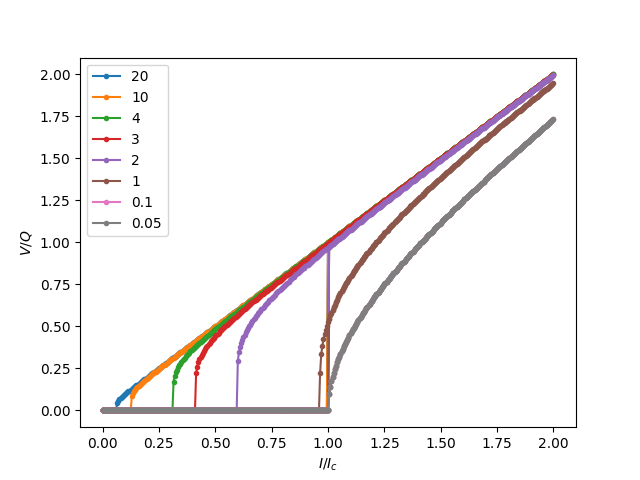
\includegraphics[width=0.5\linewidth]{../plots/ivcs_updown}
		\caption{Current-voltage curves for various damping cases.
			As predicted by theory, high damping ($Q\ll1$) corresponds to a square-root like IVC with no hysteresis, while low damping ($Q\gg1$) results in strong hystersis with a almost linear retrapping branch.}
		\label{fig:ivcsupdown}
	\end{figure}
	
	
	\section{Voltage biasing}
	
	\bibliography{bib/cited.bib}
	
\end{document}
